\begin{figure}[!htb]

    \centering

    \begin{subfigure}[b]{0.49\textwidth}
        \centering
        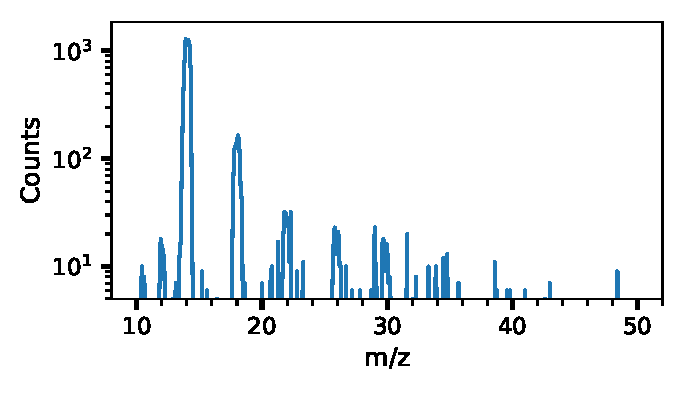
\includegraphics[width=1\textwidth]{figures/measurements/masspec/CD+_masspec_lowP_1.6e+14_4.8K.pdf}
        \caption{}
        \label{fig:masspec:lownHe}
    \end{subfigure}
    \hfill
    \begin{subfigure}[b]{0.49\textwidth}
        \centering
        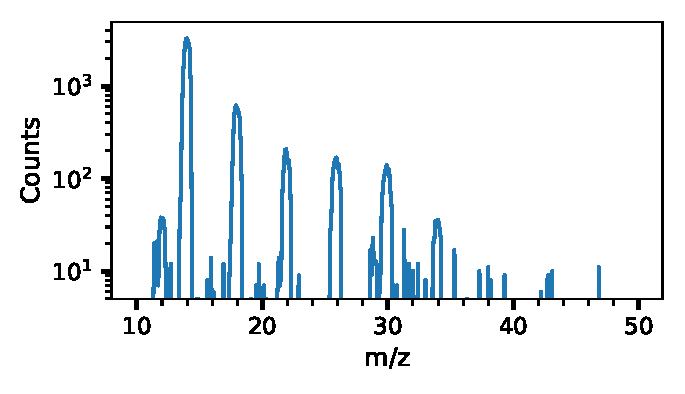
\includegraphics[width=1\textwidth]{figures/measurements/masspec/CD+_masspec_highP_2.5e+14_4.8K.pdf}
        \caption{}
        \label{fig:masspec:highnHe}
    \end{subfigure}
    
    \caption{ Measured mass spectrum after storing \CD ions (m/z $14$) for $\sim$600 ms in the cryogenic ion trap using He buffer gas (a): $1.97(7)\cdot10^{14}$~cm$^{-3}$; (b): $3.07(12)\cdot10^{14}$~cm$^{-3}$ number density at T=4.8(3)K, showing the \CD ion and the subsequent formation of ion-He complexes with up to (a): four; (b): five He atoms attached.}
    \label{fig:masspec}

\end{figure}
